% Makros zur Kompatibilitaet mit Onlinemodul: 
 \providecommand{\MoIl}[1][]{\mbox{}#1]\mathopen{}} 
 \providecommand{\MoIr}[1][]{#1[\mbox{}} 
 \providecommand{\MIntvlSep}{;} 
 \providecommand{\MElSetSep}{\, ; \, } 
 \begin{MAufgabe}{Lineare Betrags(un)gleichungen}{vr, 2016, MaTeX}
L\"osen Sie die Gleichung
$$
 \MDS 5\left| 8\, x - 2 \right|2 - 4\, x=  \left| 4\, x - 3 \right|  - 4\, x - 1
$$  

\ifLsg\MLoesung

Im ersten Schritt k\"onnen die Terme au\ss{}erhalb der Betragszeichen zusammengefasst werden:

\begin{align*} 
 5\left| 8\, x - 2 \right|2 - 4\, x=  \left| 4\, x - 3 \right|  - 4\, x - 1\\ 
\Leftrightarrow5\, \left|8\, x - 2\right| - \left|4\, x - 3\right| + 3= 0 
 \end{align*}

F\"ur diese Gleichung haben wir 4 F\"alle zu unterscheiden: 
\begin{enumerate}
\item $ \MDS 
\begin{cases} 
 0 \leq 8\, x - 2\\ 
0 \leq 4\, x - 3
 \end{cases}
\Leftrightarrow \frac{3}{4} \leq x\Leftrightarrow x \in [ \frac{3}{4} \, \MIntvlSep \, \infty\MoIr $ 
\item $ \MDS 
\begin{cases} 
 0 \leq 8\, x - 2\\ 
4\, x - 3 < 0
 \end{cases}
\Leftrightarrow x < \frac{3}{4} \wedge \frac{1}{4} \leq x\Leftrightarrow x \in [ \frac{1}{4} \, \MIntvlSep \, \frac{3}{4}\MoIr $ 
\item $ \MDS 
\begin{cases} 
 8\, x - 2 < 0\\ 
0 \leq 4\, x - 3
 \end{cases}
 \mbox{ : keine L\"osung. Diese Bedingung ist nirgendwo erf\"ullt.}$ 
\item $ \MDS 
\begin{cases} 
 8\, x - 2 < 0\\ 
4\, x - 3 < 0
 \end{cases}
\Leftrightarrow x < \frac{1}{4}\Leftrightarrow x \in \MoIl  -\infty \, \MIntvlSep \, \frac{1}{4}\MoIr $ 
\end{enumerate} 
Der 3. Fall ist nirgendwo erf\"ullt. Betrachte weiter nur die restlichen F\"alle.
 
 Fallunterscheidung: 

 \begin{enumerate} 
 \item Sei $ \MDS x\in[ \frac{3}{4} \, \MIntvlSep \, \infty\MoIr $. 
 In diesem Fall gilt: 
  $ \MDS \left| 8\, x - 2\right|=8\, x - 2$ und $ \MDS \left| 4\, x - 3\right|=4\, x - 3$. \\ 
 Damit ist die Gleichung 
 $$ 
5\, \left|8\, x - 2\right| - \left|4\, x - 3\right| + 3= 0
$$
 \"aquivalent zur Gleichung
 $$ 
5\left(8\, x - 2\right)-\left( 4\, x - 3\right)+3= 0 
$$  
$$ 
 \Leftrightarrow 36\, x - 4= 0 
$$  
$$ \Leftrightarrow x = \frac{1}{9} . 
 $$ 
 Die L\"osung muss auch die Fallbedingung $x\in [ \frac{3}{4} \, \MIntvlSep \, \infty\MoIr  $ erf\"ullen. Die gefundene L\"osung $x=\frac{1}{9}$ erf\"ullt die Fallbedingung  $x\in [ \frac{3}{4} \, \MIntvlSep \, \infty\MoIr $ nicht und deshalb ist  $$
 \mathcal{L}_{1}=\emptyset 
 $$ 
\item Sei $ \MDS x\in[ \frac{1}{4} \, \MIntvlSep \, \frac{3}{4}\MoIr $. 
 In diesem Fall gilt: 
  $ \MDS \left| 8\, x - 2\right|=8\, x - 2$ und $ \MDS \left| 4\, x - 3\right|=3 - 4\, x$. \\ 
 Damit ist die Gleichung 
 $$ 
5\, \left|8\, x - 2\right| - \left|4\, x - 3\right| + 3= 0
$$
 \"aquivalent zur Gleichung
 $$ 
5\left(8\, x - 2\right)-\left( 3 - 4\, x\right)+3= 0 
$$  
$$ 
 \Leftrightarrow 44\, x - 10= 0 
$$  
$$ \Leftrightarrow x = \frac{5}{22} . 
 $$ 
 Die L\"osung muss auch die Fallbedingung $x\in [ \frac{1}{4} \, \MIntvlSep \, \frac{3}{4}\MoIr  $ erf\"ullen. Die gefundene L\"osung $x=\frac{5}{22}$ erf\"ullt die Fallbedingung  $x\in [ \frac{1}{4} \, \MIntvlSep \, \frac{3}{4}\MoIr $ nicht und deshalb ist  $$
 \mathcal{L}_{2}=\emptyset 
 $$ 
\item Sei $ \MDS x\in\MoIl  -\infty \, \MIntvlSep \, \frac{1}{4}\MoIr $. 
 In diesem Fall gilt: 
  $ \MDS \left| 8\, x - 2\right|=2 - 8\, x$ und $ \MDS \left| 4\, x - 3\right|=3 - 4\, x$. \\ 
 Damit ist die Gleichung 
 $$ 
5\, \left|8\, x - 2\right| - \left|4\, x - 3\right| + 3= 0
$$
 \"aquivalent zur Gleichung
 $$ 
5\left(2 - 8\, x\right)-\left( 3 - 4\, x\right)+3= 0 
$$  
$$ 
 \Leftrightarrow 10 - 36\, x= 0 
$$  
$$ \Leftrightarrow x = \frac{5}{18} . 
 $$ 
 Die L\"osung muss auch die Fallbedingung $x\in \MoIl  -\infty \, \MIntvlSep \, \frac{1}{4}\MoIr  $ erf\"ullen. Die gefundene L\"osung $x=\frac{5}{18}$ erf\"ullt die Fallbedingung  $x\in \MoIl  -\infty \, \MIntvlSep \, \frac{1}{4}\MoIr $ nicht und deshalb ist  $$
 \mathcal{L}_{3}=\emptyset 
 $$ 
 \end{enumerate} 
  Die L\"osungsmenge des Ausgangsproblems ist die Vereinigung der einzelnen L\"osungsmengen: 
$$ \mathcal{L} = \mathcal{L}_{1} \cup \mathcal{L}_{2} \cup \mathcal{L}_{3} 
 = \emptyset\cup \emptyset\cup \emptyset 
   =\emptyset 
   . $$ 
 
 \begin{center}
 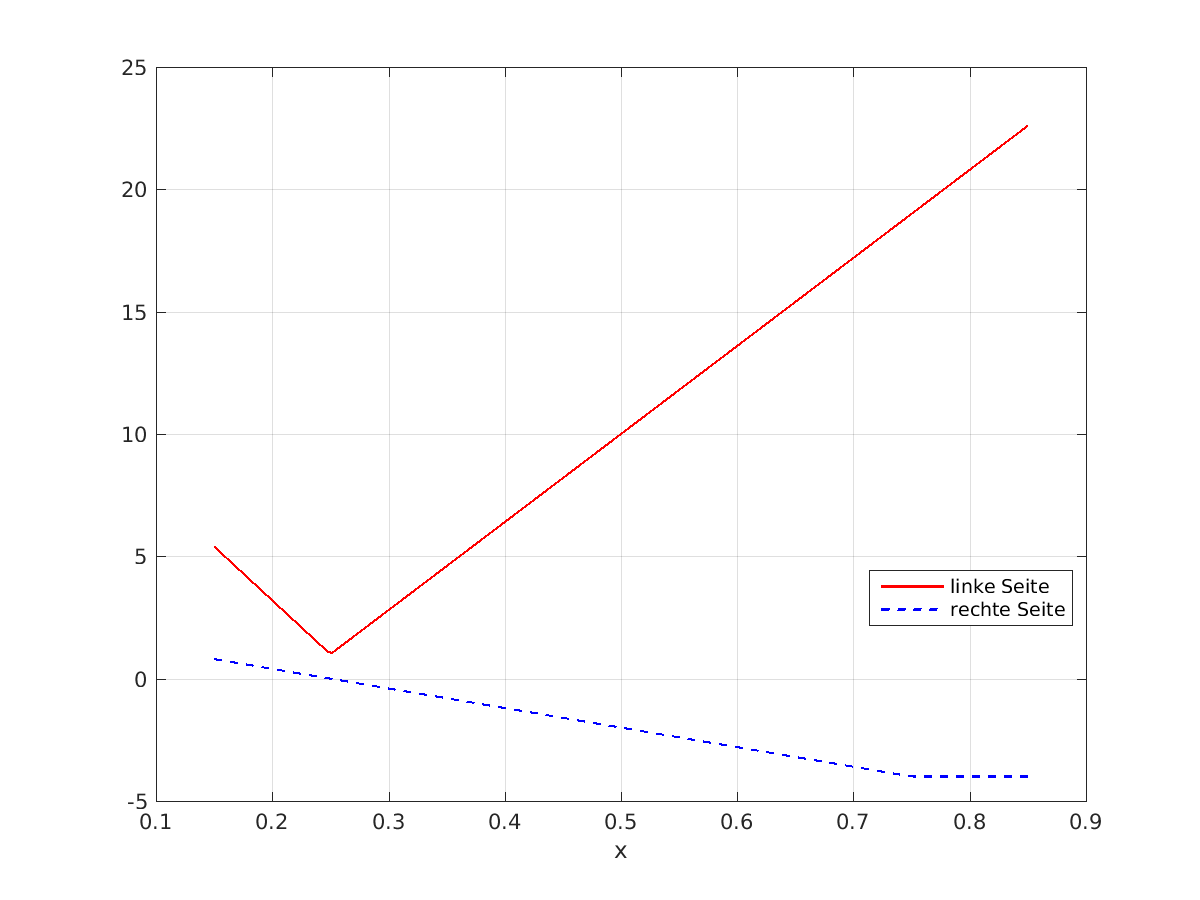
\includegraphics[width=0.8\linewidth]{Abb_zur_Ag_autogenerated_ineq_4.png} \end{center}
 
\else\relax\fi
 \end{MAufgabe}